\PassOptionsToPackage{unicode=true}{hyperref} % options for packages loaded elsewhere
\PassOptionsToPackage{hyphens}{url}
\documentclass[12pt,ignorenonframetext,aspectratio=169]{beamer}
\IfFileExists{pgfpages.sty}{\usepackage{pgfpages}}{}
\setbeamertemplate{caption}[numbered]
\setbeamertemplate{caption label separator}{: }
\setbeamercolor{caption name}{fg=normal text.fg}
\beamertemplatenavigationsymbolsempty
\usepackage{lmodern}
\usepackage{amssymb}
\usepackage{amsmath}
\usepackage{ifxetex,ifluatex}
\usepackage{fixltx2e} % provides \textsubscript
\ifnum 0\ifxetex 1\fi\ifluatex 1\fi=0 % if pdftex
  \usepackage[T1]{fontenc}
  \usepackage[utf8]{inputenc}
\else % if luatex or xelatex
  \ifxetex
    \usepackage{mathspec}
  \else
    \usepackage{fontspec}
\fi
\defaultfontfeatures{Ligatures=TeX,Scale=MatchLowercase}






%
\fi

  \usetheme[]{iqss}






% use upquote if available, for straight quotes in verbatim environments
\IfFileExists{upquote.sty}{\usepackage{upquote}}{}
% use microtype if available
\IfFileExists{microtype.sty}{%
  \usepackage{microtype}
  \UseMicrotypeSet[protrusion]{basicmath} % disable protrusion for tt fonts
}{}


\newif\ifbibliography


\hypersetup{
      pdftitle={Factor-factor relationship},
        pdfauthor={Deependra Dhakal},
          pdfborder={0 0 0},
    breaklinks=true}
%\urlstyle{same}  % Use monospace font for urls







% Prevent slide breaks in the middle of a paragraph:
\widowpenalties 1 10000
\raggedbottom

  \AtBeginPart{
    \let\insertpartnumber\relax
    \let\partname\relax
    \frame{\partpage}
  }
  \AtBeginSection{
    \ifbibliography
    \else
      \let\insertsectionnumber\relax
      \let\sectionname\relax
      \frame{\sectionpage}
    \fi
  }
  \AtBeginSubsection{
    \let\insertsubsectionnumber\relax
    \let\subsectionname\relax
    \frame{\subsectionpage}
  }



\setlength{\parindent}{0pt}
\setlength{\parskip}{6pt plus 2pt minus 1pt}
\setlength{\emergencystretch}{3em}  % prevent overfull lines
\providecommand{\tightlist}{%
  \setlength{\itemsep}{0pt}\setlength{\parskip}{0pt}}

  \setcounter{secnumdepth}{0}


  \usepackage{booktabs}
  \usepackage{longtable}
  \usepackage{emptypage}
  \usepackage{array}
  \usepackage{multirow}
  \usepackage{wrapfig}
  \usepackage{float}
  \usepackage{colortbl}
  \usepackage{pdflscape}
  \usepackage{tabu}
  \usepackage{threeparttable}
  \usepackage{threeparttablex}
  \usepackage[normalem]{ulem}
  \usepackage{rotating}
  \usepackage{makecell}
  \usepackage{xcolor}
  \usepackage{tikz} % required for image opacity change
  \usepackage[absolute,overlay]{textpos} % for text formatting
  \usepackage[utf8]{inputenc}
  \usetikzlibrary{mindmap,arrows,shapes,positioning,shadows,trees}

  % this font option is amenable for beamer
  \setbeamerfont{caption}{size=\tiny}


%% IQSS overrides
\iqsssectiontitle{Outline}

\AtBeginSection[]{
  \title{\insertsectionhead}
  {
    \definecolor{white}{rgb}{0.776,0.357,0.157}
    \definecolor{iqss@orange}{rgb}{1,1,1}
    \ifnum \insertmainframenumber > \insertframenumber
    \frame{
      \frametitle{\iqsssectiontitleheader}
      \tableofcontents[currentsection]
    }
    \else
    \frame{
      \frametitle{Backup Slides}
      \tableofcontents[sectionstyle=shaded/shaded,subsectionstyle=shaded/shaded/shaded]
    }
    \fi
  }
}

\AtBeginSubsection[]{}

%%


  \title[]{Factor-factor relationship}



  \author[
        Deependra Dhakal
    ]{Deependra Dhakal}

  \institute[
    ]{
    GAASC, Baitadi \and Tribhuwan University
    }

\date[
      \today
  ]{
      \today
        }

\begin{document}

% Hide progress bar and footline on titlepage
  \begin{frame}[plain]
  \titlepage
  \end{frame}



\hypertarget{introduction}{%
\section{Introduction}\label{introduction}}

\begin{frame}{Background}
\protect\hypertarget{background}{}
\begin{itemize}
\tightlist
\item
  Production function or factor-product relationship deals only with one
  output and one variable input; all other inputs being considered
  fixed.
\item
  Actually there are many situations where there a large number of
  inputs which are used to produce a farm commodity.
\item
  The farmers are faced with the problem of deciding about the use of
  more than one resource or set of resources in substitution of other
  resources or set of resources.
\item
  For example, it is common problem with the farmer to decide on how
  much of N, P and K fertilizer to use with a view to getting certain
  level of a crop output.
\item
  Same problem applies to livestock rearing where how much of
  concentrates and green foodders to feed the milch animal to get
  certain amount of milk should be decided.
\end{itemize}
\end{frame}

\begin{frame}{Substitution}
\protect\hypertarget{substitution}{}
\begin{itemize}
\tightlist
\item
  There is possibility of substituting one factor (\(X_1\)) for another
  (\(X_2\)) as product level (Y) is held constant.
\item
  Thus objectives of analysis of factor-factor relationship are:

  \begin{enumerate}
  \tightlist
  \item
    Minimization of cost at a given level of output
  \item
    Optimization of output to the fixed factors through alternative
    resource-use combinations
  \end{enumerate}
\item
  In context of factor-factor substitution involving only two factors,
  adding more of a quantity of factor \(X_1\) while replacing the amount
  of \(X_2\) is referred to as factor \(X_1\) substituting factor
  \(X_2\).
\end{itemize}
\end{frame}

\begin{frame}{Example}
\protect\hypertarget{example}{}
\begin{itemize}
\tightlist
\item
  Let us suppose a farmer is producing wheat with various combinations
  of two fertilizer inputs -- Nitrogenous fertilizer and Phosphatic
  fertilizer. At various levels of input combinations, we obtains
  quanitites of output as shown in Table \ref{tab:np-factor-factor}.
\end{itemize}

\begin{table}

\caption{\label{tab:np-factor-factor}Combination of inputs resulting in different levels of output.}
\centering
\fontsize{6}{8}\selectfont
\begin{tabular}[t]{rrrrrrr}
\toprule
phosphorus & nitrogen 40 & nitrogen 60 & nitrogen 80 & nitrogen 100 & nitrogen 120 & nitrogen 140\\
\midrule
\rowcolor{gray!6}  40 & 40 & 43 & 45 & 45 & 44 & 44\\
60 & 42 & 46 & 48 & 49 & 49 & 48\\
\rowcolor{gray!6}  80 & 41 & 45 & 48 & 50 & 51 & 51\\
\bottomrule
\end{tabular}
\end{table}
\end{frame}

\begin{frame}{Isoquant or iso-product curve}
\protect\hypertarget{isoquant-or-iso-product-curve}{}
\begin{itemize}
\tightlist
\item
  An isoquant curve represents the various input combinations that can
  be used to produce a given output.
\item
  Each point on an isoquant is the maximum output that can be produced
  with these input combinations.
\item
  For example, suppose 80, 108 and 120 units of output (yield of wheat
  per ropani of land) can be produced using the following input
  combinations (nitrogen (\(X_1\)) and phosphorus (\(X_2\)) fertilizer
  in kg per ropani):
\end{itemize}
\end{frame}

\begin{frame}{}
\protect\hypertarget{section}{}
\begin{figure}

{\centering 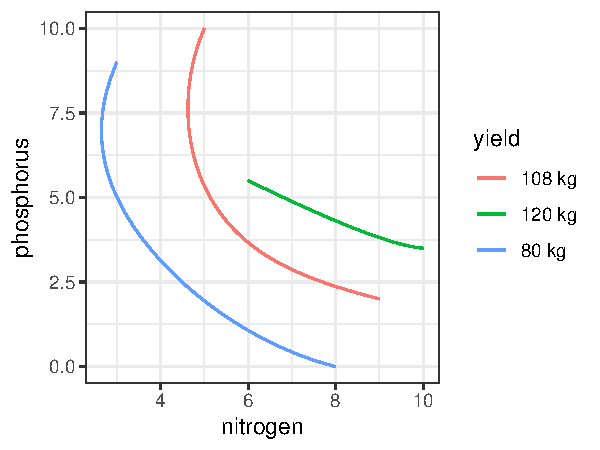
\includegraphics[width=0.4\linewidth]{05-factor_factor_relationship_files/figure-beamer/np-factor-factor-output-1} 

}

\caption{Isoquant curves showing combination of various level of inputs to produce different level of outputs}\label{fig:np-factor-factor-output}
\end{figure}
\end{frame}

\begin{frame}{}
\protect\hypertarget{section-1}{}
Suppose a farmer has Rs 10000 of fund outlay for fertilizer purchase.
His budget line for purchase of Nitrogen and Phosphorus fertilizer
purchase is shown in Figure \ref{fig:budget-line-fertilizer}.

\begin{figure}
\includegraphics[width=0.45\linewidth]{05-factor_factor_relationship_files/figure-beamer/budget-line-fertilizer-1} \caption{Budget line for outlay of Rs 10000 for fertilizer purchase at Rates of Rs 30 per kg for Nitrogen fertilizer and Rs 50 per kg for Phosphorus fertilizer.}\label{fig:budget-line-fertilizer}
\end{figure}
\end{frame}

\begin{frame}{}
\protect\hypertarget{section-2}{}
\begin{itemize}
\tightlist
\item
  We can show the isoquant lines of using those two inputs in various
  combinations to produce different levels of Wheat yield (kg). The
  least cost combination of inputs with outlay of Rs 10000 is shown in
  Figure \ref{fig:least-cost-combination}.
\end{itemize}

\begin{figure}
\includegraphics[width=0.45\linewidth]{05-factor_factor_relationship_files/figure-beamer/least-cost-combination-1} \caption{Least cost combination of two factors for Wheat production}\label{fig:least-cost-combination}
\end{figure}
\end{frame}

\begin{frame}{}
\protect\hypertarget{section-3}{}
\begin{itemize}
\tightlist
\item
  Isoquants can be traced to different level of outputs. We can imagine
  that there is an isoquant for every output level between and including
  lowest and highest production level.
\item
  The Figure \ref{fig:np-factor-factor-output} shows the isoquant map of
  three isoquant curves.
\end{itemize}
\end{frame}

\begin{frame}{Properties of isoquants}
\protect\hypertarget{properties-of-isoquants}{}
\begin{itemize}
\tightlist
\item
  Isoquants, like indifference curves, slope downward form left to right
  (i.e.~have negative slope)
\item
  No to isoquants can intersect each other
\item
  Isoquants, like indifference curves, are convex to the origin; this
  implies the diminishing returns to a variable factor.
\end{itemize}
\end{frame}

\hypertarget{types-of-factor-factor-relationships}{%
\section{Types of factor-factor
relationships}\label{types-of-factor-factor-relationships}}

\begin{frame}{}
\protect\hypertarget{section-4}{}
\begin{itemize}
\tightlist
\item
  The shapes of the isoquants and production surface will depend upon
  the manner in which the variable inputs are combined to produce a
  particular level of output.
\item
  There can be 3 categories of such combinations of inputs:

  \begin{enumerate}
  \tightlist
  \item
    Fixed proportion combination of inputs
  \item
    Constant rate of substitution, and
  \item
    Varying rates of substitution
  \end{enumerate}
\end{itemize}
\end{frame}

\begin{frame}{Fixed proportion combination}
\protect\hypertarget{fixed-proportion-combination}{}
\begin{itemize}
\tightlist
\item
  There are certain enterprises or products which can only be produced
  if inputs are added in fixed proportion at all levels of production.
\item
  In this case there is no decision problem because the inputs combine
  in fixed proportion.
\item
  An example situation is that of tractor-driver combination. Adding
  another tractor will necessitate addition of a driver too.
\item
  Inputs combining in fixed proportions give rise to L-shaped isoquants.
\end{itemize}

\begin{table}[H]
\centering
\begin{tabular}{lrr}
\toprule
yield & tractor & driver\\
\midrule
\rowcolor{gray!6}  2 tons & 1 & 1\\
3 tons & 3 & 3\\
\rowcolor{gray!6}  4 tons & 4 & 4\\
\bottomrule
\end{tabular}
\end{table}
\end{frame}

\begin{frame}{}
\protect\hypertarget{section-5}{}
\begin{block}{Marginal rate of substitution}
\protect\hypertarget{marginal-rate-of-substitution}{}
\begin{itemize}
\tightlist
\item
  The rate at which two inputs can be substituted at a given level of
  output called MRS.
\item
  It is denoted as: \(\frac{\Delta X_2}{\Delta X_1}\).
\end{itemize}
\end{block}
\end{frame}

\begin{frame}{Constant rate of substitution}
\protect\hypertarget{constant-rate-of-substitution}{}
\begin{itemize}
\tightlist
\item
  The substitution at constant rate occurs when the amount of one input
  replaced by the other point does not change as the added input
  increases in magnitude.
\item
  The isoquant of such combination is a straight line.
\item
  For inputs which can be exchanged at a constant rate, the slope of the
  product contour is constant, or in other words, the substitution ratio
  remains same.
\end{itemize}

\[
\frac{\Delta X_{21}}{\Delta X_{11}} = \frac{\Delta X_{22}}{\Delta X_{12}} = \frac{\Delta X_{23}}{\Delta X_{13}} = ... = \frac{\Delta X_{2n}}{\Delta X_{1n}}
\]
\end{frame}

\begin{frame}{}
\protect\hypertarget{section-6}{}
\begin{table}[H]
\centering
\begin{tabular}{lrr}
\toprule
yield & women labor & men labor\\
\midrule
\rowcolor{gray!6}  2 tons & 10 & 1\\
2 tons & 8 & 2\\
\rowcolor{gray!6}  2 tons & 6 & 3\\
2 tons & 4 & 4\\
\rowcolor{gray!6}  2 tons & 2 & 5\\
\bottomrule
\end{tabular}
\end{table}
\end{frame}

\begin{frame}{Varying rate of substitution}
\protect\hypertarget{varying-rate-of-substitution}{}
\begin{itemize}
\tightlist
\item
  There can be increasing rate of substitution on decreasing rate of
  substitution. It can also be the case that MRS changes from increasing
  initially to decreasing finally and vice versa.
\item
  Substitution at increasing rate is rarely available in agriculture,
  but the substitution at decreasing rate is more common in agriculture.
\item
  Decreasing rate of substitution means that every subsequent increase
  in the use of one factor replaces less and less of the other.
\item
  Examples are substitution among concentrates and green fodder, labour
  and capital, and nitrogen and phosphorus, etc.
\end{itemize}
\end{frame}

\begin{frame}{}
\protect\hypertarget{section-7}{}
\begin{table}[H]
\centering
\begin{tabular}{lrrrrr}
\toprule
Yield & Nitrogen ($X_2$) & Phosphorus ($X_1$) & $\Delta X_2$ & $\Delta X_1$ & MRS ($\frac{\Delta X_2}{\Delta X_1}$)\\
\midrule
\rowcolor{gray!6}  2 tons & 46 & 0 &  &  & \\
2 tons & 32 & 2 & -14 & 2 & 7.0\\
\rowcolor{gray!6}  2 tons & 20 & 4 & -12 & 2 & 6.0\\
2 tons & 10 & 6 & -10 & 2 & 5.0\\
\rowcolor{gray!6}  2 tons & 1 & 8 & -9 & 2 & 4.5\\
\addlinespace
2 tons & 0 & 10 & -1 & 2 & 0.5\\
\bottomrule
\end{tabular}
\end{table}
\end{frame}

\hypertarget{cost-minimization}{%
\section{Cost minimization}\label{cost-minimization}}

\begin{frame}{Isocost line (price line/budget line/iso-outlay
line/factor cost line)}
\protect\hypertarget{isocost-line-price-linebudget-lineiso-outlay-linefactor-cost-line}{}
\begin{itemize}
\tightlist
\item
  All possible combination of two inputs which can be purchased with a
  given outlay or budget.
\end{itemize}

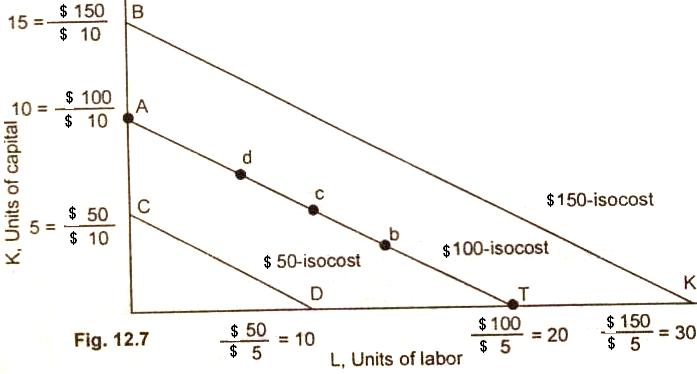
\includegraphics[width=0.45\linewidth]{./figs/isocost-line-budget-outlay-shift}
\end{frame}

\begin{frame}{}
\protect\hypertarget{section-8}{}
\textbf{Important points regarding isocost line}:

\begin{itemize}
\tightlist
\item
  As the total outlay increases the isocost line moves farther away from
  the origin.
\item
  Isocost line is straight line because input prices do not change with
  the quantity purchased.
\item
  The slope of isocost line indicates the ratio of factor prices.
\end{itemize}
\end{frame}

\begin{frame}{Least cost combination of inputs}
\protect\hypertarget{least-cost-combination-of-inputs}{}
\begin{itemize}
\tightlist
\item
  There are innumerable possible combination of factors which can be
  used to produce a particular level of output. The problem is to find
  out the combination of inputs which should cost the least, a cost
  minimization problem.
\item
  There are three methods to find out the least cost combination of
  inputs.

  \begin{itemize}
  \tightlist
  \item
    Arithmetic method
  \item
    Algebraic method
  \item
    Graphical method
  \end{itemize}
\end{itemize}
\end{frame}

\begin{frame}{Arithmetic method}
\protect\hypertarget{arithmetic-method}{}
\begin{itemize}
\item
  One possible way to determine the least cost combination is to compute
  the cost of all possible combinations of inputs and then select one
  combination with minimum cost. This method is suitable where only a
  few combination produce a particular level of output.
\item
  Suppose price of input1 is Rs 3 and the price of input2 is Rs 2.
\end{itemize}

\begin{tabular}{rrrrr}
\toprule
Input 1 & Input 2 & Input 1 Cost & Input 2 Cost & Total Cost\\
\midrule
10 & 3 & 30 & 6 & 36\\
7 & 4 & 21 & 8 & 29\\
5 & 6 & 15 & 12 & 27\\
3 & 8 & 9 & 16 & 25\\
2 & 12 & 6 & 24 & 30\\
\bottomrule
\end{tabular}
\end{frame}

\begin{frame}{}
\protect\hypertarget{section-9}{}
The above table shows 5 combinations of inputs which can produce a given
level of output. The total cost of each combination of inputs is
computed. Out of 5 combinations, 3 units of input1 and 8 units of input2
is the least combination of inputs. i.e.~Rs. 25.
\end{frame}

\begin{frame}{Algebraic method (Steps)}
\protect\hypertarget{algebraic-method-steps}{}
\begin{enumerate}
\tightlist
\item
  Compute marginal rate of technical substitution
\end{enumerate}

\[MRS = \frac{\textrm{Number of units of replaced resources}}{\textrm{Number of units of added resources}}\]

or,

\[MRS(X_1 \textrm{ for } X_2) = \frac{\Delta X_2}{\Delta X_1}\] and,

\[MRS(X_2 \textrm{ for } X_1) = \frac{\Delta X_1}{\Delta X_2}\]
\end{frame}

\begin{frame}{}
\protect\hypertarget{section-10}{}
\begin{enumerate}
\setcounter{enumi}{1}
\tightlist
\item
  Compute price ratio (PR)
\end{enumerate}

\[PR = \frac{\textrm{Price per unit of added resource}}{\textrm{Price per unit of replaced resource}}\]

So,

\[PR = \frac{P_{X_1}}{P_{X_2}}\] if \(MRS(X_1 \textrm{ for } X_2)\), and

\[PR = \frac{P_{X_2}}{P_{X_1}}\] if \(MRS(X_2 \textrm{ for } X_1)\)
\end{frame}

\begin{frame}{}
\protect\hypertarget{section-11}{}
\begin{enumerate}
\setcounter{enumi}{2}
\tightlist
\item
  Work out the least cost combination by equating MRS and PR. i.e.,
\end{enumerate}

\[
\frac{\Delta X_2}{\Delta X_1} = \frac{P_{X_1}}{P_{X_2}}
\]

or,

\[
\frac{\Delta X_1}{\Delta X_2} = \frac{P_{X_2}}{P_{X_1}}
\]

\begin{itemize}
\tightlist
\item
  The least cost combination is obtained when, \(MRS = PR\)
\end{itemize}
\end{frame}

\begin{frame}{Graphical method}
\protect\hypertarget{graphical-method}{}
\begin{itemize}
\item
  Since the slope of isoquant indicates Marginal Rate of Technical
  Substitution (MRTS) and the slope of isocost line indicates factor
  price ratio, minimum cost for given output will be indicated by point
  of tangency between these two lines.
\item
  Isocost and isoquant lines are drawn on the same graph for different
  levels of production. The least cost combination will be at the point
  where isocost line is tangent to the isoquant; i.e.~MRS = PR
\end{itemize}
\end{frame}

\hypertarget{isocline-ridge-lines-and-expansion-path}{%
\section{Isocline, ridge lines and expansion
path}\label{isocline-ridge-lines-and-expansion-path}}

\begin{frame}{Isocline}
\protect\hypertarget{isocline}{}
\begin{itemize}
\tightlist
\item
  There can be number of possible output levels as shown in figure
  \ref{fig:isocline-expansion-path} and least cost combination can be
  found out for these various output levels.
\end{itemize}

\begin{figure}
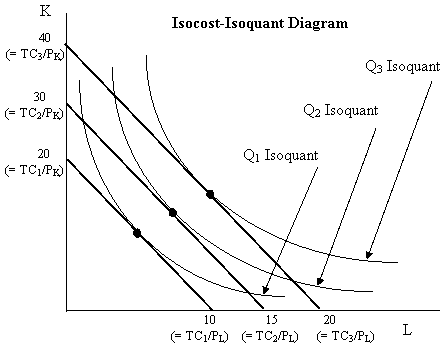
\includegraphics[width=0.45\linewidth]{./figs/Isoquant_isocost_graph} \caption{Isoquant and isocost lines for different levels of output}\label{fig:isocline-expansion-path}
\end{figure}
\end{frame}

\begin{frame}{}
\protect\hypertarget{section-12}{}
\textbf{Features of isocline}

\begin{itemize}
\tightlist
\item
  Isocline passess through all isoquants at points where they have same
  slope
\item
  It shows how the relative proportion of the factors changes as the
  output is increased.
\item
  It shows that resources should be used along this line as long as MVP
  \textgreater{} MC of resources used.
\end{itemize}
\end{frame}

\begin{frame}{Ridge lines}
\protect\hypertarget{ridge-lines}{}
\begin{itemize}
\tightlist
\item
  Represents the points of maximum output from each input, given a fixed
  amount of the other input.
\item
  On the ridge lines MPP is zero.
\item
  Ridge lines represent the region of economic relevance.
\item
  Within the ridge lines MPP of both inputs is positive but decreasing.
\end{itemize}
\end{frame}

\begin{frame}{Expansion path}
\protect\hypertarget{expansion-path}{}
\begin{itemize}
\tightlist
\item
  The line or curve connecting the points of least cost combination for
  different levels of output is called expansion path. Expansion path is
  an isocline on which slope of isoquant (MRTS) equal the slopes of
  isocost line (Price ratio).
\item
  The expansion path indicates the best way of producing the different
  levels of output given the input prices and the technology.
\item
  If expansion path is a straight line through origin, it means inputs
  will be used in the same proportion at all output levels and hence it
  is called scale line. -It is curved; it implies the inputs will be
  used in various proportions.
\end{itemize}
\end{frame}




\end{document}
